\section{Data Representations \& Processing}

The goal of this section is to introduce the idea of data representations and one general method to represent data. We will also study different data processing techniques and introduce the problem of class imbalance and solutions to address it.

\begin{parag}{Recap: What data?}
	Let us first remember what data we are talking about when talking about machine learning, data can be:
	\begin{itemize}
	    \item Attributes
	    \item Text
	    \item Sound
	    \item Images
	\end{itemize}
\end{parag}
	The problem with data is that it can be very \important{heterogeneous} for instance:
	\begin{center}
		\fbox{
		\begin{minipage}{0.9\linewidth}
		I am looking for an inexpensive motorcycle, nothing fancy, have to be able to do all maintenance my self.\\ 
		$ $\\
		Looking in the <\$400 range. If you can help me out, GREAT!, please reply by e-mail.
		\end{minipage}
	}

	\end{center}
	\begin{center}
		\fbox{
		\begin{minipage}{0.9\linewidth}
		Whoops!! Wrong group.  Soooooooooooooooooorry folks..
		\end{minipage}
	}
	\end{center}
	\begin{center}
		\fbox{
		\begin{minipage}{0.9\linewidth}
		I'd like to see this info as well. As for wavelength, I think you're primarily going to find two - 880 nM +/- a bit, and/or 950 nM +/- a bit. Usually it is about 10 nM either way. The two most common I have seen were 880 and 950 but I have also heard of 890 and 940. I'm not sure that the 10 nM one way or another will make a great deal of difference. Another suggestion - find a brand of TV that uses an IR remote, and go look at the SAMS photofact for it. You can often find some very detailed schematics and parts list for not only the receiver but the transmitter as well, including carrier freq. specs. and tone decoding specs. if the system uses that.
		\end{minipage}
	}
	\end{center}
	
	As you can see, here this become pretty hard to vectorize right? How can we leverage text documents of different length? With linear model, the number of parameter depends directly of the input dimensions.\\
	$ $\\
	The same goes for image. Let us have two images one of size $536 \times 356 \times 3$ and the other of size $500 \times 500 \times 3$. First we have the same issue as before (both image doesn't have the same dimensionality). Second, the size of the dimension input is enormous, for the first image we are in $x_i \in \mathbb{R}^{536 \times 356 \times 3} = \mathbb{R}^{572448}$. Now let us have a big dataset i.e. one million images and this becomes just too big for us. We need data representations.
	

\subsection{Data representations: Attributes}
One way in order to represent data is to use attributes, let us take the example of UCI Abalone dataset which predict the age of abalone from measurements. The attributes are:
\begin{center}
\begin{tabular}{|c|c|c|c|}
	\hline
	Name & Data Type & Measurement & Description \\
	\hline
	Sex & Categorical & & M, F, and I (infant) \\
	\hline
	Length & Numeric (continuous) & mm &  Longest shell measurements\\
	\hline
	Diameter & Numeric (continuous) & mm &  perpendicular to length\\
	\hline
	Height & Numeric (continuous) & mm &  with meat in shell\\
	\hline
	WT\_Whole & Numeric (continuous) & grams &  whole abalone\\
	\hline
	WT\_Shuck & Numeric (continuous) & grams &  weight of meat\\
	\hline
	WT\_Vscra & Numeric (continuous) & grams &  gut weight\\
	\hline
	WT\_Shell & Numeric (continuous) & grams &  after being dried\\
	\hline
	Rings & Numeric (integer) &  & +1.5 gives the age in years \\
	\hline
\end{tabular}
\end{center}
As we can see we can have: categorical attributes (like a label), real (continuous), integer (discrete). What is good however with attributes is that all input have the same number of attributes.\\
$ $\\
Going back to the text examples from above, let us try to represent our data! First we have to see some common point between all input, all samples are written in the same language $\implies$ they relate to the same dictionary. The idea is that for each sample, we count the number of times each word in the dictionary appears. For instance:

	\begin{center}
		\fbox{
		\begin{minipage}{0.9\linewidth}
			(1) John likes to watch movies. Mary likes movies too.
		\end{minipage}
	}
	\end{center}
	
	\begin{center}
		\fbox{
		\begin{minipage}{0.9\linewidth}
			(2) John also likes to watch football games.
		\end{minipage}
	}
	\end{center}
	
	The corresponding counts gives us:
	\begin{itemize}
		\item BoW1 = \{"\textit{John}":1,"\textit{likes}":2, "\textit{to}":1, "\textit{watch}":1, "\textit{movies}":2, "\textit{Mary}":1, "\textit{too}":1\}
		\item BoW2 = \{"\textit{John}":1,"\textit{also}":1,"\textit{likes}":1, "\textit{to}":1, "\textit{watch}":1, "\textit{football}":1, "\textit{games}":1\}
	\end{itemize}
	We don't need to have the whole English dictionary so what we will do is to take all word that are in both texts (union) and remove the common words, e.g. "\textit{the}", "\textit{a}", "\textit{to}"...\\
	$ $\\
	With $D$ words in the dictionary, each samples can be represented as a vector in $\mathbb{R}^{D}$, Using the dictionary we made above ($D = 9$):
	\begin{align*} 
		\widetilde{x}_1 = \begin{pmatrix} 1 & 2 & 1 & 2 & 1 & 1 & 0 & 0 & 0 \end{pmatrix} \\
		\widetilde{x}_2 =  \begin{pmatrix} 1 & 1 & 1 & 0 & 0 & 0 & 1 & 1 & 1 \end{pmatrix} 
	\end{align*}
	But here you could guess that for text sample of different length, the actual word counts may not be relevant (longer texts will just have larger values). Instead, we will encode the proportion of each word, this is achieved by dividing each vector element by the sum of all elements. Our $\widetilde{x}_1$ has a total sum equals to $\sum_{d= 1}^{D}\widetilde{x}_1^{\left(d\right)}= 8$. The final representation of this text is therefore:
	\begin{align*} 
		x_1 = \begin{pmatrix} \frac{1}{8} & \frac{1}{4} & \frac{1}{8} & \frac{1}{4} & \frac{1}{8} & \frac{1}{8} & 0 & 0 & 0 \end{pmatrix} 
	\end{align*}
	In essence, what we are doing is computing the frequency of each words in our text.
	

	\paragraph{How about images}%
	\label{par:How about images}
	When trying to create attributes for images we have a big problem, there is no direct notion of '\textit{words}' for image data. However, objects are made of common parts/patches. The goal here is therefore to extract the patches from all images and to create a \important{visual dictionary} of those parts:
	\begin{center}
	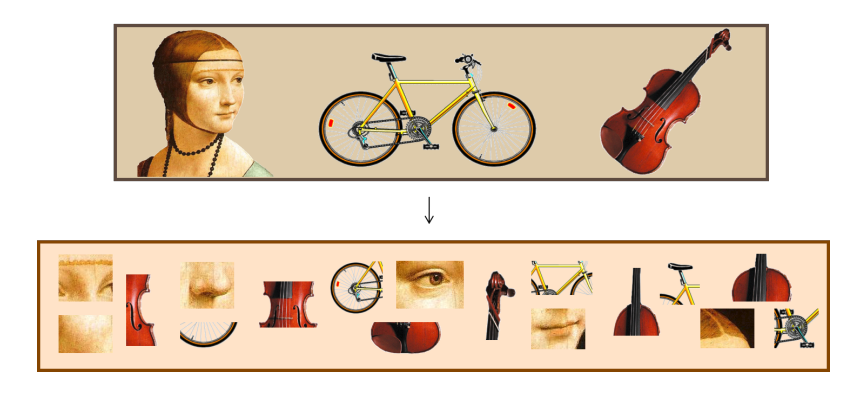
\includegraphics[scale=0.3]{screenshots/2026-04-13.png}
	\end{center}
	In order to create this dictionary, we will have to group the patches based on similarity to obtain prototypes that act as dictionary words. To do so we will use Clustering algorithm.
	\begin{center}
	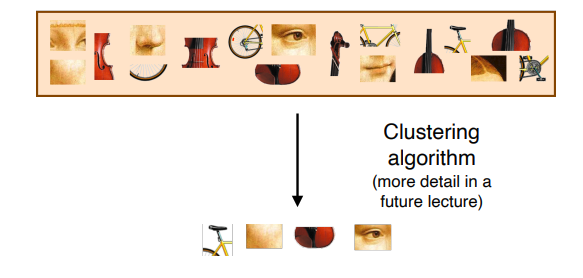
\includegraphics[scale=0.3]{screenshots/2026-04-13_1.png}
	\end{center}
	The center of each cluster (group) is taken as a visual word
	\begin{parag}{Bag of visual words}
		For each patch in an image:
		\begin{itemize}
		    \item find the nearest visual word
		    \item add one to the corresponding element in a BoW vector
		\end{itemize}
		Normalize the BoW vectors to obtain histograms
	\end{parag}
	\begin{center}
	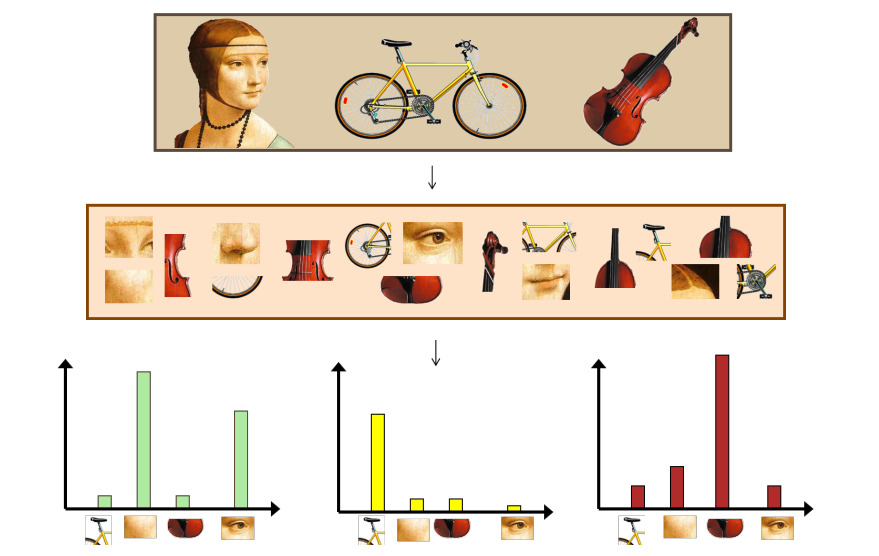
\includegraphics[scale=0.3]{screenshots/2026-04-13_2.png}
	\end{center}
	This still requires comparing local image patches 
	\begin{itemize}
	    \item The patches can all have the same size
	    \item They can be small enough for this to be manageable
	\end{itemize}
	However this is not great as there is a lot of noise and intensity issues. There is other local image representations which can be used (which goes beyond the scope of this course).


	\begin{parag}{Conclusion}
		Large, heterogeneous data can be made compact and homogeneous.\\
		$ $\\
		The resulting representations can be directly used as input to a machine learning algorithm.
		\begin{itemize}
		    \item This is applicable to all the methods we have seen so far
		    \item But in general to most machine learning algorithms
		\end{itemize}
		
	    
	\end{parag}
	


\subsection{Data pre-processing}
Even with a good representation, the data might benefit from being pre processed. This is because:
\begin{itemize}
	\item Some attribute values are missing
    \item Some attribute values are noisy
    \item The feature dimensions are of incommensurate magnitude
\end{itemize}

\begin{parag}{Missing data}
    For instance let us assume that some attribute values were not recorded (e.g. the Air quality UCI dataset contains missing values, which are tagged with a -200 value)
	\begin{subparag}{Potential solutions}
		\begin{itemize}
			\item Ignore the corresponding
			\item Fill in the missing values with global constant
			\item Fill in the missing values with the corresponding attribute average over the dataset
			\item Fill in the missing values with the corresponding attribute average over the samples belonging to the same class
		\end{itemize}
		
	\end{subparag}
\end{parag}


\begin{parag}{Noisy data}
    Noisy data can come from a lot of reasons, for instance random measurement error, faulty data collection, data entry problem \ldots But our algorithm is not made for that "\textit{dirty}" data, we need to \important{clean} it.\\
	$ $\\
	A way of doing that is called \important{binning} which works like this:
	\begin{itemize}
	    \item For each attribute:
			\begin{enumerate}
				\item Sort the data
				\item Partition it into bins
				\item Smooth the data by taking the bin means, or medians
			\end{enumerate}
	\end{itemize}
	Another way is \important{clustering}, we detect outliers as the clusters with too few elements and remove these samples.
\end{parag}
\begin{parag}{Data Normalization}
    The goal of this technique is to scale each individual attribute/feature dimension to fall within a specified range
	\begin{subparag}{Min-max normalization}
	    For each feature dimension $d$, compute the normalized feature:
		\begin{align*} 
			\widetilde{x}_i^{\left(d\right)} = \frac{x_i^{\left(d\right)}-x_{min}^{\left(d\right)}}{x_{max}^{\left(d\right)}-x_{min}^{\left(d\right)}}
		\end{align*}
		Where
		\begin{align*} 
			x_{min}^{\left(d\right)} &= \overset{N}{\min_{i= 1}} \; x_i^{\left(d\right)}\\
			x_{max}^{\left(d\right)} &= \overset{N}{\max_{i= 1}} \; x_i^{\left(d\right)}
		\end{align*}
	\end{subparag}
	\begin{subparag}{x-score normalization}
	    For each feature dimension $d$, compute the normalized feature
		\begin{align*} 
			\widetilde{x}_{i}^{\left(d\right)} =  \frac{d_i^{\left(d\right)} - \mu^{\left(d\right)}}{\sigma^{\left(d\right)}}
		\end{align*}
		Where 
		\begin{align*} 
			\mu^{\left(d\right)} &= \frac{1}{N} \sum_{i= 1}^{N}x_i^{\left(d\right)}\\
							\sigma^{\left(d\right)}	 &= \sqrt{\frac{1}{N}\sum_{i= 1}^{N}\left(x_i^{\left(d\right)} - \mu^{\left(d\right)}\right)^2}
		\end{align*}
	\end{subparag}
	\begin{subparag}{max normalization}
	    For each feature dimension $d$, compute the normalized feature:
		\begin{align*} 
			\widetilde{x}_i^{\left(d\right)} = \frac{x_i^{\left(d\right)}}{x_{max}^{\left(d\right)}}
		\end{align*}
		Where 
		\begin{align*} 
			x_{max}^{\left(d\right)} =  \overset{N}{\max_{i= 1}}\left|x_i^{\left(d\right)}\right|
		\end{align*}
	\end{subparag}
	\begin{subparag}{Normalization by decimal scaling}
	    For each feature dimension $d$, compute the normalized feature 
		\begin{align*} 
			\widetilde{x}_i^{\left(d\right)} = \frac{x_^{\left(d\right)}}{10^{k}}
		\end{align*}
		Where $k$ is the smallest integer such that 
		\begin{align*} 
			\overset{N}{\max_{i= 1}} \left|\widetilde{x}_i^{\left(d\right)}\right| \leq 1
		\end{align*}
	\end{subparag}
	For all data processing techniques, the normalized (or cleaned) features are then used as input to a machine learning algorithm.\\
	$ $\\
	Normalization is not always necessary, and may or may not help depending on the data at hand on the chosen machine learning algorithm.
\end{parag}

\begin{parag}{From data sample to data set}
    Data representations and data cleaning/normalization acts on the individual samples 
	\begin{itemize}
	    \item Although the normalization statistics come from the whole training set
	\end{itemize}
	Nevertheless, even with good representations, the data set itself might make from learning more difficult.
\end{parag}

A good illustration of this can be imbalanced data. I remember a meme I saw online on a model that output whether or not a number was a prime number in $\Theta\left(1\right)$, it was:
\begin{lstlisting}[language=python]
def isPrime(n):
	return True
\end{lstlisting}
As you can see this '\textit{model}' is very fast and almost always correct but it misses the whole point of the model right? The reason for this is that the data is so imbalanced that assuming it always on label gives us a good accuracy.


\begin{center}
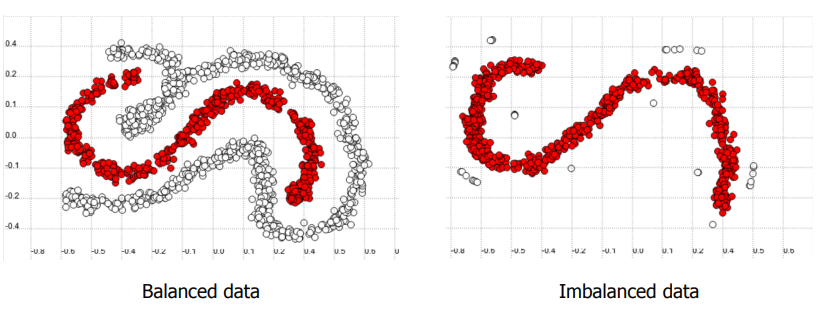
\includegraphics[scale=0.3]{screenshots/2026-04-13_3.png}
\end{center}

\begin{parag}{Learning with imbalanced data}
    In order to have a model that still work, there is two main approaches, one act on the \important{data}: Sampling Methods, the other act on the cost function: Cost Sensitive Methods.
\end{parag}
\begin{parag}{Sampling methods}
    The issue we are facing here is the lack of data, in order to compensate we can either increase the data set by generating new data points for the smallest class, or decrease the dataset by removing redundant data points from the largest class.
	\begin{subparag}{Decrease the data: Undersampling}
	    Here we will have naive (random) undersampling:
		\begin{itemize}
		    \item Randomly remove samples from the largest class until you obtain a balanced data set
		\end{itemize}
		However this may remove important samples\\
		$ $\\
		A more clever undersampling would be to remove the data point that we '\textit{don't need}' -- the redundant samples. Imagine that we have two data points that are almost identical $\implies$ removing one doesn't change much the distribution of the data. This methods is good if the class to undersample is densely populated (e.g. low-dimensional representation because of the curse of dimensionality)
	\end{subparag}
	\begin{subparag}{Increase the data: Oversampling}
	    Here again we can use the naive (random) oversampling:
		\begin{itemize}
		    \item Replicate the data samples from the smallest class until you obtain a balanced data set
		\end{itemize}
		The drawbacks here is that this may lead to overfitting\\
		$ $\\
		A more clever oversampling would be to create new data points based on neighbouring existing ones, meaning we take to sample and create a new one in the middle $\implies$ can lead to create noisy samples.
	\end{subparag}
	However there is a lot of other method to oversampling:
	\begin{itemize}
		\item SMOTE: Synthetic minority oversampling technique (CHawla et al., JAIR 2002)
		\item AdaSyn: Adaptive synthetic sampling (HE et al., IJCNN 2008)
		\item Reason about the density of data points and the border with other class
	\end{itemize}
\end{parag}
\begin{center}
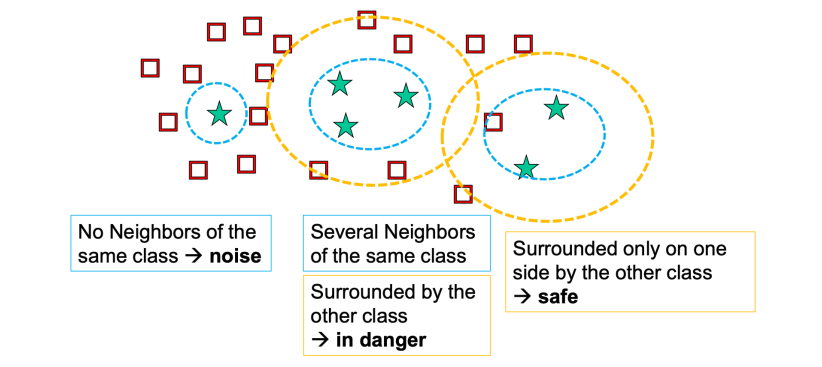
\includegraphics[scale=0.4]{screenshots/2026-04-13_4.png}
\end{center}
Now let us go to the other side with Cost Sensitive Methods.

\begin{parag}{Empirical risk}
    Given $N$ training samples $\left\{\left(x_, y_i\right)\right\}$, the empirical risk is defined as  
	\begin{align*} 
		R\left(\{x_i\}, \{y_i\}, w\right) = \frac{1}{N}\sum_{i= 1}^{N}l\left(\hat{y}_i , y_i\right)
	\end{align*}
	Where $\left\{x_i\right\}$ and $\left\{y_i\right\}$ are the sets of training inputs and labels, respectively.\\
	$ $\\
	In general, each loss term $l\left(\hat{y}_i , y_i\right)$ has the same influence. With imbalanced data, this means that most of the empirical risk comes from the largest class. A simple solution to this problem consist of re-weighting the samples, to put more emphasis on the rare class. This gives an empirical risk of the form 
	\begin{align*} 
		R\left(\{x_i\}, \{y_i\}, w\right) = \frac{1}{N}\sum_{i= 1}^{N}\beta_i l\left(\hat{y}_i , y_i\right)
	\end{align*}
	where $\beta_i$ is the weight for sample $i$
	\begin{subparag}{Remark}
		Note that $\beta_i$ cannot be optimized, because the optimal solution would simply be to set all of them to $0$. Instead they are manually, e.g., inversely proportional to the class frequency:
		\begin{align*} 
			\beta_i = 1 - \frac{N_K}{N}
		\end{align*}
		If sample $i$ belongs to class $k$, which contains $N_K$ samples
	\end{subparag}
	This strategy is quite general, it can apply to the least-square classification:
	\begin{align*} 
		\min_{w} \sum_{i= 1}^{N}\beta_i \left\|W^{T}x_i - y_i\right\|^2 + \lambda \left\|W\right\|_F^2
	\end{align*}
	Logistic regression 
	\begin{align*} 
		\min_W = -\sum_{i= 1}^{N}\beta_i \sum_{k= 1}^{C}y_i^{\left(k\right)}\ln\left(w_{\left(k\right)}^{T}x_i\right)
	\end{align*}
	And also support vector machines 
	\begin{align*} 
		\min_{\omega^{\left(0\right)}, \widetilde{W}}\frac{1}{2C}\left\|\widetilde{W}\right\|^2 + \sum_{i= 1}^{N}\beta_i \max\left(0, 1 - y_i \cdot \left(w^{\left(0\right)} + \widetilde{w}^{T}x_i\right)\right)
	\end{align*}
	In the three cases, since the weights are fixed during optimization, the respective optimization problems remain convex and can thus be solved to optimality
\end{parag}


\begin{parag}{From handcrafted representations to learned ones}
    The representations and data processing strategies we have discussed so far were all manually designed. There is, however no guarantee that they are the best representations for the task at hand. \\
	$ $\\
	Ideally, one would therefore like to learn the representation jointly with the classifier. This will bring us to the topic of artificial neural networks.
\end{parag}











	
	
	
